%----------createOperationInClass----------------------------------------
\op
{createOperationInClass}
{creates a new operation in a class}
{createOperationInClass(Class selectedEObject, String nameValue, Class typeValue)}
{The class providing the container for the newly created operation.} {
\begin{itemize}
 \item nameValue/newName: The name of the newly created operation
 \item idValue/newID: The id of the newly created operation
 \item typeValue/newType: The type of the newly created operation
\end{itemize}
}
{There is no operation in the same context whose name equals the parameter-value
of 'newName' (see
\ref{subsec:checkOtherNames})}
{Only the name and the id will be set via input data. Visibility, isAbstract adn
isStatic will be set with a default value as defined with the diagram editor in
the image below. The 'newType' input data is a concrete propagated class.}
\begin{figure}[H]
  \centering
  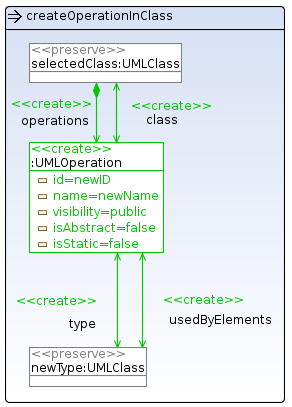
\includegraphics[width=0.45\textwidth]{pics/createOperationInClass.png}
  \caption{createOperationInClass}
  \label{createOperationInClass}
\end{figure}
%----------createOperationInInterface----------------------------------------
\op
{createOperationInInterface}
{creates a new operation in an interface}
{createOperationInInterface(Interface selectedEObject, String nameValue, Class typeValue)}
{The interface providing the container for the newly created
operation.} {
\begin{itemize}
 \item nameValue/newName: The name of the newly created operation
 \item idValue/newID: The id of the newly created operation
 \item typeValue/newType: The type of the newly created operation
\end{itemize}
}
{There is no operation in the same context whose name equals the parameter-value
of 'newName' (see
\ref{subsec:checkOtherNames})}
{Only the name and the id will be set via input data. Visibility, isAbstract adn
isStatic will be set with a default value as defined with the diagram editor in
the image below. The 'newType' input data is a concrete propagated interface.}
\begin{figure}[H]
  \centering
  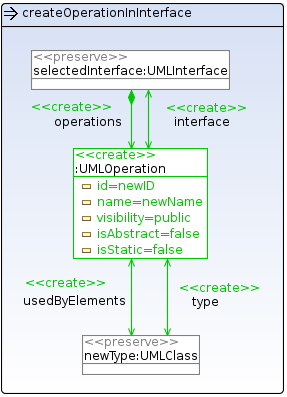
\includegraphics[width=0.45\textwidth]{pics/createOperationInInterface.png}
  \caption{createOperationInInterface}
  \label{createOperationInInterface}
\end{figure}
%----------deleteOperation----------------------------------------
\op
{deleteOperation}
{Deletes an operation}
{deleteOperation(Operation selectedEObject)}
{The operation which should be deleted} {-}
{-}
{For a better readability this is a simplified version of the
'deleteOperation'-transformation and will only cover cases where the operation
has no containments and no references to other elements. Such a complex
transformation rule exits but won't be listed here.
\\\\In this simplified version we have three rules. One that checks if the
container of the operation is a model and the other rules that deletes the
operation depending on the found container type. In the following image of the
units you can see the case distinction done with a Conditional Unit. We assume
the container is an interface if not a class.}
\begin{figure}[H]
\advance\leftskip-1.5cm
  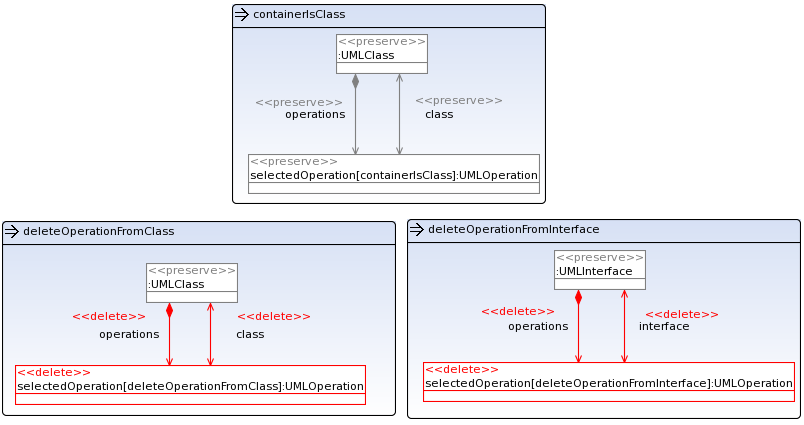
\includegraphics[width=1.2\textwidth]{pics/deleteOperation_emptyAndUnreferenced.png}
  \caption{deleteOperation}
  \label{deleteOperation}
\end{figure}

\begin{figure}[H]
  \centering
  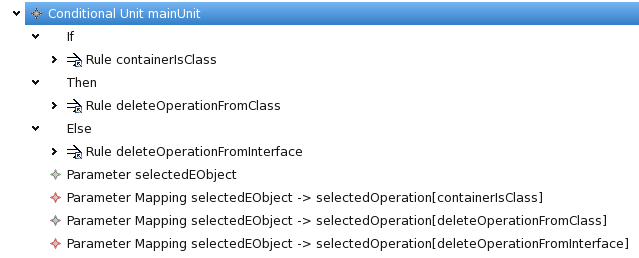
\includegraphics[width=1.0\textwidth]{pics/deleteOperation_emptyAndUnreferenced_TreeView.png}
  \caption{deleteOperation(UnitView)}
  \label{deleteOperation(UnitView)}
\end{figure}
%----------editOperationName----------------------------------------
\op
{editOperationName}
{edits the name of an operation}
{editOperationName(Operation selectedEObject, String nameValue)}
{The operation whose name should be renamed.}
{
\begin{itemize}
 \item nameValue/newName: The new name
\end{itemize}
}
{There is no operation in the same class whose name equals the parameter-value of
'newName' (see
\ref{subsec:checkOtherNames})}
{The \textless\textless create\textgreater\textgreater  -symbol in the image
means that even if the attribute exists its value will be overwritten.
'someName' is the placeholder for the input name.}
\begin{figure}[H]
  \centering
  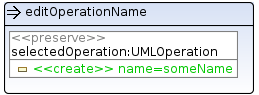
\includegraphics[width=0.4\textwidth]{pics/editOperationName.png}
  \caption{editOperationName}
  \label{editOperationName}
\end{figure}
%----------editOperationIsAbstract----------------------------------------
\op
{editOperationIsAbstract}
{edits the isAbstract-value of an operation}
{editOperationIsAbstract(Operation selectedEObject, boolean booleanValue)}
{The operation whose isAbstract-value should be edited.}
{
\begin{itemize}
 \item booleanValue/bool: The new isAbstract-value
\end{itemize}
}
{The \textless\textless create\textgreater\textgreater  -symbol in the image
means that even if the attribute exists its value will be overwritten.
'bool' is the placeholder for the input boolean value.}
{safsdfsd}
\begin{figure}[H]
  \centering
  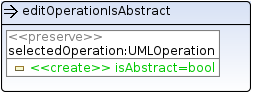
\includegraphics[width=0.4\textwidth]{pics/editOperationIsAbstract.png}
  \caption{editOperationIsAbstract}
  \label{editOperationIsAbstract}
\end{figure}
%----------editOperationIsStatic----------------------------------------
\op
{editOperationIsStatic}
{edits the isStatic-value of an operation}
{editOperationIsStatic(Operation selectedEObject, boolean booleanValue)}
{The operation whose isStatic-value should be edited.}
{
\begin{itemize}
 \item booleanValue/bool: The new isStatic-value
\end{itemize}
}
{-}
{The \textless\textless create\textgreater\textgreater  -symbol in the image
means that even if the attribute exists its value will be overwritten.
'bool' is the placeholder for the input boolean value.}
\begin{figure}[H]
  \centering
  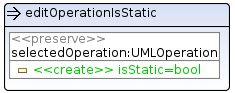
\includegraphics[width=0.4\textwidth]{pics/editOperationIsStatic.png}
  \caption{editOperationIsStatic}
  \label{editOperationIsStatic}
\end{figure}
%----------editOperationVisibility----------------------------------------
\op
{editOperationVisibility}
{edits the visibility of an operation}
{editOperationVisibility(Operation selectedEObject, Visibility visibilityValue)}
{The operation whose visibility should be edited.}
{
\begin{itemize}
 \item visibilityValue/visibility: The new visiblility
\end{itemize}
}
{-}
{The \textless\textless create\textgreater\textgreater  -symbol in the image
means that even if the attribute exists its value will be overwritten.
'visibility' is the placeholder for the input visibility value.}
\begin{figure}[H]
  \centering
  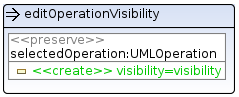
\includegraphics[width=0.4\textwidth]{pics/editOperationVisibility.png}
  \caption{editOperationVisibility}
  \label{editOperationVisibility}
\end{figure}
%----------editOperationReturnTypeFromClassToClass----------------------------------------
\op
{editOperationReturnTypeFromClassToClass}
{edits the type of an operation from a class to another}
{editOperationReturnTypeFromClassToClass(Operation selectedEObject, Class typeValue)}
{The operation whose type should be edited.}
{
\begin{itemize}
 \item typeValue/newType: The new type
\end{itemize}
}
{-}
{Only references will change.}
\begin{figure}[H]
  \centering
  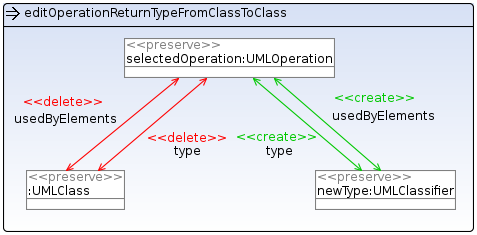
\includegraphics[width=0.8\textwidth]{pics/editOperationReturnTypeFromClassToClass.png}
  \caption{editOperationReturnTypeFromClassToClass}
  \label{editOperationReturnTypeFromClassToClass}
\end{figure}
%----------editOperationReturnTypeFromClassToPrimitive----------------------------------------
\op
{editOperationReturnTypeFromClassToPrimitive}
{edits the type of an operation from a class to a primitiveType}
{editOperationReturnTypeFromClassToPrimitive(Operation selectedEObject, PrimitiveType typeValue)}
{The operation whose type should be edited.}
{
\begin{itemize}
 \item typeValue/newType: The new type
\end{itemize}
}
{-}
{Only references will change.}
\begin{figure}[H]
  \centering
  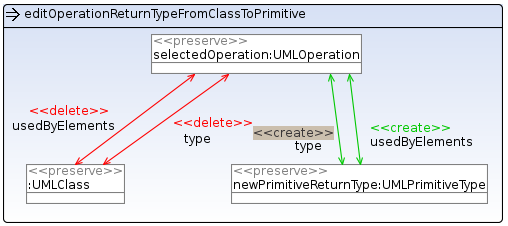
\includegraphics[width=0.8\textwidth]{pics/editOperationReturnTypeFromClassToPrimitive.png}
  \caption{editOperationReturnTypeFromClassToPrimitive}
  \label{editOperationReturnTypeFromClassToPrimitive}
\end{figure}
%----------editOperationReturnTypeFromPrimitiveToClass----------------------------------------
\op
{editOperationReturnTypeFromPrimitiveToClass}
{edits the type of an operation from a primitiveType to a class}
{editOperationReturnTypeFromPrimitiveToClass(Operation selectedEObject, Class typeValue)}
{The operation whose type should be edited.}
{
\begin{itemize}
 \item typeValue/newType: The new type
\end{itemize}
}
{-}
{Only references will change.}
\begin{figure}[H]
  \centering
  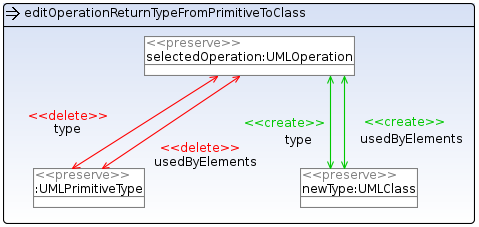
\includegraphics[width=0.8\textwidth]{pics/editOperationReturnTypeFromPrimitiveToClass.png}
  \caption{editOperationReturnTypeFromPrimitiveToClass}
  \label{editOperationReturnTypeFromPrimitiveToClass}
\end{figure}
%----------editOperationReturnTypeFromPrimitiveToPrimitive----------------------------------------
\op
{editOperationReturnTypeFromPrimitiveToPrimitive}
{edits the type of an operation from a primitiveType to a primitiveType}
{editOperationReturnTypeFromPrimitiveToPrimitive(Operation selectedEObject, PrimitiveType typeValue)}
{The operation whose type should be edited.} {
\begin{itemize}
 \item typeValue/newType: The new type
\end{itemize}
}
{-}
{Only references will change.}
\begin{figure}[H]
  \centering
  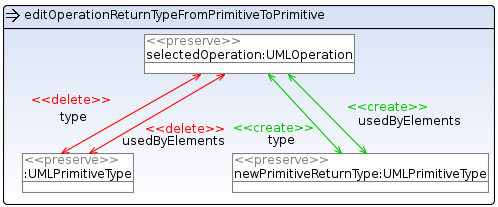
\includegraphics[width=0.8\textwidth]{pics/editOperationReturnTypeFromPrimitiveToPrimitive.png}
  \caption{editOperationReturnTypeFromPrimitiveToPrimitive}
  \label{editOperationReturnTypeFromPrimitiveToPrimitive}
\end{figure}
%----------moveOperationBetweenClasses----------------------------------------
\op
{moveOperationBetweenClasses}
{moves an operation from a class to another class}
{moveOperationBetweenClasses(Operation selectedEObject, Class tgt)}
{The operation which should be moved.}
{
\begin{itemize}
 \item tgt/tgtClass: the target class
\end{itemize}
}
{There is no operation with the same name in the target context (see
\ref{subsec:checkOtherNames})}
{Only references change.}
\begin{figure}[H]
  \centering
  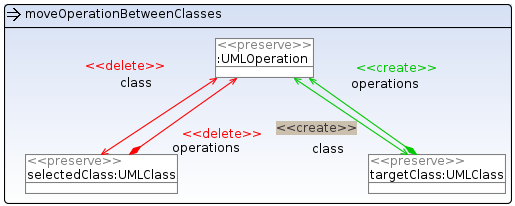
\includegraphics[width=0.8\textwidth]{pics/moveOperationBetweenClasses.png}
  \caption{moveOperationBetweenClasses}
  \label{moveOperationBetweenClasses}
\end{figure}
%----------moveOperationBetweenInterfaces----------------------------------------
\op
{moveOperationBetweenInterfaces}
{moves an operation from an interface to another}
{moveOperationBetweenInterfaces(Operation selectedEObject, Interface tgt)}
{The operation which should be moved.}
{
\begin{itemize}
 \item tgt/targetInterface: the target interface
\end{itemize}
}
{There is no operation with the same name in the target context (see
\ref{subsec:checkOtherNames})}
{Only references change.}
\begin{figure}[H]
  \centering
  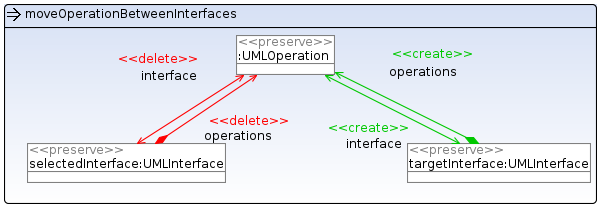
\includegraphics[width=0.9\textwidth]{pics/moveOperationBetweenInterfaces.png}
  \caption{moveOperationBetweenInterfaces}
  \label{moveOperationBetweenInterfaces}
\end{figure}
%----------moveOperationFromClassToInterface----------------------------------------
\op
{moveOperationFromClassToInterface}
{moves an operation from a class to an interface}
{moveOperationFromClassToInterface(Operation selectedEObject, Interface tgt)}
{The operation which should be moved.}
{
\begin{itemize}
 \item tgt/targetInterface: the target interface
\end{itemize}
}
{There is no operation with the same name in the target context (see
\ref{subsec:checkOtherNames})}
{Only references change.}
\begin{figure}[H]
  \centering
  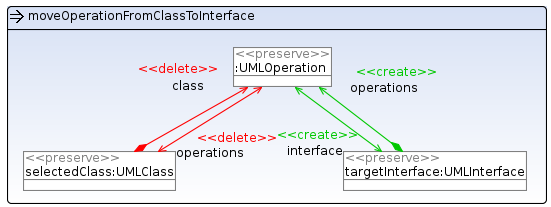
\includegraphics[width=0.9\textwidth]{pics/moveOperationFromClassToInterface.png}
  \caption{moveOperationFromClassToInterface}
  \label{moveOperationFromClassToInterface}
\end{figure}
%----------moveOperationFromInterfaceToClass----------------------------------------
\op
{moveOperationFromInterfaceToClass}
{moves an operation from an interface to a class}
{moveOperationFromInterfaceToClass(Operation selectedEObject, Class tgt)}
{The operation which should be moved.}
{
\begin{itemize}
 \item tgt/targetClass: the target class
\end{itemize}
}
{There is no operation with the same name in the target context (see
\ref{subsec:checkOtherNames})}
{Only references change.}
\begin{figure}[H]
  \centering
  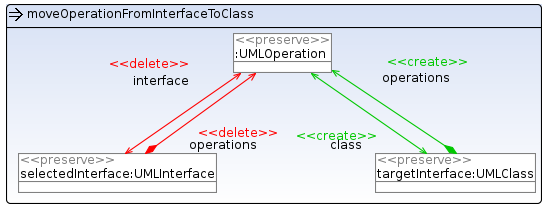
\includegraphics[width=0.9\textwidth]{pics/moveOperationFromInterfaceToClass.png}
  \caption{moveOperationFromInterfaceToClass}
  \label{moveOperationFromInterfaceToClass}
\end{figure}